\cotefile{81}
\scanpage{49}
\unsure{$R$|$\mathcal{R}$} relation d'\unsure{équiva|équiv.} non \unsure{panachée|ponctuelle} sur $S$.

\uline{Segments} \inserted{$\underline{R}$} \uline{saturés} : \unsure{stable|stables} par passage au complémentaire, et par intersection et réunion quand celles-ci \deleted{\unsure{d}}donnent des segments (\inserted{p. ex. si} $A\cup B\ne S$, $A\cap B\ne\varnothing$)

Si $S_i\in\unsure{\mathcal{R}|R}$, alors les segments composants de $\complement S_i$ sont saturés, donc aussi leurs complémentaires i.e. les segments minimaux contenant $S_i$ (ou \inserted{segments} cocomposants de $S_i$). \deleted{Plus \unsure{général\textsuperscript{mt}|généralement}, si $T\subset S$ est une partie de $S$ $R$-saturée, alors les segments composants de}

\noindent\llap{\rule[-.92\baselineskip]{.4pt}{1.8\baselineskip}\hspace{.35em}}\uline{Prop} Les segments saturés minimaux sont les $\deleted{\unsure{A|S}}S_i\in R$ qui sont des segments.

% slanted
\reversemarginpar\margin{On appelle \unsure{les|ces} parties des \uline{onglets}}

Il est évident que si $S_i\in\deleted{\unsure{A}}R$ est un segment, alors c'est un segment saturé, et il est minimal parmi ces derniers (et $=$ parmi les parties saturées non vides). Inversement, soit $A$ segment saturé minimal, \deleted{\unsure{soit}} soit $S_i\in R$, $S_i\subset A$, \deleted{soit} je dis que $S_i=A$, \deleted{\unsure{ou|sin}} i.e. que l'on ne peut avoir $S_i,S_j\in R$ distincts, et
% slanted
\margin{\unsure{moitié|motif|mettant} du côté de la \unsure{section|notion|notation}}
\par\noindent\begin{minipage}[t]{.23\linewidth}
\vspace{0pt}
\figure{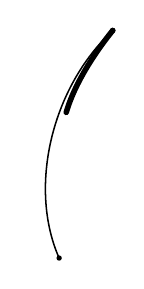
\begin{tikzpicture}[x=1cm,y=1cm,line cap=round,line join=round]
  \draw[line width=.55pt] (0.15,0) .. controls (-.24,.88) and (.04,2.15) .. (.83,2.89);
  \draw[line width=2pt] (.24,1.85) .. controls (.35,2.23) and (.62,2.63) .. (.83,2.89);
  \fill (.15,0) circle (.034) (.83,2.89) circle (.036);
\end{tikzpicture}}


\end{minipage}\hfill\begin{minipage}[t]{.73\linewidth}
\vspace{0pt}
$\subset A$. En effet, si $A_i$ $(A_j)$ est le \unsure{segm|segm.} cocomposant de $\deleted{\unsure{A}}S_i$ qui est contenu dans $A$, alors la condition que $S_i,S_j$ sont \deleted{\unsure{dis}}\unsure{non|bien} panachés s'exprime par la condition que $A_i\cap A_j=\varnothing$, donc $A_i,A_j$ sont des segments saturés $\subset A$ et $\ne A$, absurde.
\end{minipage}
\normalmarginpar
% archive sheet number: 48

\scanpage{50}
\uline{Cor} Tout \deleted{\unsure{conti|cont}} segment saturé contient un onglet -- donc si $\unsure{\mathcal{R}|R}$ n'est pas la relation grossière il existe au moins deux onglets (car il existe alors au moins deux segments saturés, complémentaires l'un de l'autre)

Soit \inserted{$\unsure{\Sigma_{1}|\Sigma_{0}}$ l'un des onglets de $R$,} $\deleted{\unsure{S_{0}|S_1}}\unsure{T_{1}|T_{0}}$ la réunion des onglets, $\deleted{\unsure{S_1}}R_1$ son complémentaire. Alors, si $\deleted{S_1}R_1\ne\varnothing$, $\deleted{S_1}R_1$ a au moins deux segments composants ($\operatorname{card}\unsure{\pi_0|\Pi_0}(R_1)\geq 2$), sinon $R_1$ serait un \deleted{\unsure{s}}segment donc contiendrait un onglet, absurde. Si $\operatorname{card} R_1=2$, alors $R_1\in\mathcal{R}$ \deleted{est un} donc $\mathcal{R}$ consiste en les onglets et en $R_1$, (car \deleted{\unsure{$R_1$}} \unsure{les} $S_i\subset R_1$ sont de card. $\geq 2$, \deleted{\unsure{puis|puisq}} car ceux de cardinal $1$ seraient des onglets \ldots)

Si $\operatorname{card} R_1\geq 3$, $R_1$ est lui $=$ un graphe polygonal, et $\mathcal{R}_1=\mathcal{R}\vert R_1$ est une relation d'équivalence non \unsure{panachée|panachèe}. De plus, \deleted{\unsure{al|Au}}Aucun $\unsure{S_i|S_1}\in\mathcal{R}_1$ n'est contenu dans un segment composant de $R_1$ -- sinon il serait contenu dans un segment saturé contenu dans $\deleted{\unsure{S_1}}R_1$ (\unsure{Savoir|savoir} son cocomposant contenu dans ce composant), lequel contiendrait un onglet $\subset R_1$ -- absurde. Si $\mathcal{R}_1$ est la relation grossière, on a fini -- $\mathcal{R}$ est \unsure{formée|formé} des onglets, et de $R_1$.
% margin note written sideways
\margin{\unsure{Dessin|Dossier} \unsure{plié|pliée} \illegible{1}}
% archive sheet number: 49

\scanpage{51}
Sinon, considérons l'un des \inserted{$\unsure{\mathcal{R}_1|R_1}$-}onglets, \deleted{\unsure{dis}} -- il y en a au moins deux. \inserted{Aussi l'un de} ces onglets \unsure{sont|est|seront} en corr. $1$-$1$. avec un ens. de \unsure{(}segments $\Sigma_2$ de $S$, dont chacun contient un composant au moins de $\deleted{S_1}T_1$, et dont les extrémités sont (\deleted{\unsure{di|dis}}distinctes et) dans $S_1$, et qui \unsure{sont} mutuellement disjoints. Soit $T_2$

\diagram{$\begin{array}{ccccc}\Sigma_1&\Sigma_2&\Sigma_3&-&\Sigma_i\\[3pt]T_1&T_2&T_3&&T_i\end{array}$}

$\Sigma_i$ est un ens. de segments \inserted{($R$-saturés)} mutuellement disjoints, $\operatorname{card}\Sigma_i\geq 2$, \unsure{$\cdot$|.} de réunion $T_i'$ \inserted{(\uline{NB} les \unsure{segm.|segmts} composants de $T_i$ sont donc des réunions partielles de $\Sigma_i$, donc saturés)}

\reversemarginpar\margin{\deleted{$i\unsure{\geq|\to}$}} \[T_i=T_i'\cup T_{\unsure{i-1|i}}\] \margin{$i\geq 2$ \deleted{\unsure{donc}}}\noindent\llap{\rule[-2\baselineskip]{.4pt}{3\baselineskip}\hspace{.4em}}\deleted{Tout élément $A\in\Sigma_{i-1}$ est contenu dans un $\deleted{\unsure{A}}B\in\Sigma_i$, \unsure{les|tout}}

Tout $B\in\Sigma_i$ contient au moins un \deleted{$A\in\Sigma_{i-1}$}\inserted{\uline{segment composant}} \deleted{\unsure{de}} de $T_{i-1}$, et $\partial B\subset S\setminus T_{i-1}$ \deleted{$\unsure{\partial B|B}$}\normalmarginpar

\noindent\begin{minipage}[t]{.46\linewidth}
$\Sigma_1$ ens de segments \unsure{mut\textsuperscript{t}|mut\textsuperscript{lt}} disj. de $S=S_0$, \deleted{de cardinal} \inserted{$\operatorname{card}(\Sigma_1)\geq 2$} \[T_1=\bigcup_{A\in\Sigma_1} A,\quad S_1=S\setminus T_1\] \[\deleted{\operatorname{card}S_1\geq\unsure{3|2}}\] les segm. comp. de $S_1$ dans $S$ au \unsure{nb|nbre} au moins $2$
\end{minipage}\hfill\begin{minipage}[t]{.51\linewidth}
$\Sigma'_2$ ens de segm. mut. disjoints \uline{de $S_{\unsure{2|1}}$}, \uline{non} \uline{contenus} dans un des segments composants \[\begin{aligned}\operatorname{card}\Sigma_{\unsure{1|2}}&\geq 2,\\ T_2&=T_1\cup\mathop{\deleted{\Sigma}\bigcup}\limits_{A\in\Sigma'_2} A\\ \deleted{\unsure{\Sigma}}S_2&=S\setminus T_2\\ \operatorname{card}\unsure{\pi_0|\Pi_0}(S_2)&\ne 1\end{aligned}\]
\end{minipage}
% archive sheet number: 50

\scanpage{52}
$I$ \unsure{graphe-segment} (fini) ayant au moins deux sommets

Deux \unsure{parties|paires} d'éléments $\unsure{\varepsilon|\xi},\varepsilon'\in\unsure{\mathcal{P}_2|\mathfrak{P}_2}(I)$ sont dites \uline{non \unsure{panachées}} si \inserted{$\varepsilon\cap\varepsilon'=\varnothing$ et si} $I_{\varepsilon}\cap I_{\varepsilon'}=\varnothing$ \inserted{ou $I_{\varepsilon}\subset I_{\varepsilon'}$ \uline{ou} $I_{\varepsilon'}\subset I_{\varepsilon}$}, -- $I_{\varepsilon}$ est le segment déterminé par \unsure{un|l'} ens. à deux éléments $\varepsilon$.

Deux parties $A,A'$ de $I$ sont dites non panachées si \[\begin{aligned}\text{a)}\quad&A\cap A'=\varnothing\\ \text{b)}\quad&\forall\,\varepsilon\in\mathcal{P}_2(A),\quad\varepsilon'\in\mathcal{P}_2(A'),\quad \varepsilon,\varepsilon'\ \text{non panachés}\end{aligned}\]

% slanted
\reversemarginpar\margin{ou encore, que l'un des deux $A,B$ est contenu dans un segment qui ne rencontre pas l'autre} Cela revient au \unsure{$=$} de dire que $A'$ est contenu dans l'un des \deleted{\unsure{intervalles}}\inserted{segments} composants de $I\setminus A$ \uline{ou} (si $A$ ne contient pas d'extrémité de $I$) dans la réunion des deux compos. \deleted{\unsure{de|des}} \unsure{extrêmes|extremes} (i.e. ceux qui contiennent \unsure{?} les deux extrémités

% slanted
\margin{\uline{NB} un segment peut être réduit à un seul sommet --}\normalmarginpar

Partitions non \unsure{panachées} de $I$

Ens \inserted{$\Sigma$} de segments de $I$ \unsure{spécial|qui soit} :

a) Si $A,B\in\Sigma$, on a $A\cap B=\varnothing$, ou $A\subset B$ ou $B\subset A$

b) Si $A,B\in\Sigma$, $\deleted{\unsure{A|B}}\unsure{B\subsetneq A|B\notin A}$, alors $B\cap\partial A=\varnothing$

c) \deleted{\unsure{$\forall$|$\forall\varepsilon$}}\unsure{On a|on a} $\partial I\subset\bigcup\limits_{A\in\Sigma} A$ donc $\partial I\subset\bigcup\limits_{A\in\Sigma}\partial A$

Pour un tel $\Sigma$, posons pour $A\in\Sigma$ \[ A^{\ast}=A\setminus\bigcup_{\substack{B\in\Sigma\\B\subset A}} B \qquad (\supset\partial A) \] \margin{donc $A^{\ast}\ne\varnothing$}

alors \deleted{les $A^{\ast}$, \unsure{s\textsuperscript{t}|à} deux à \unsure{de|deux}} pour $A,B\in\Sigma$, $A\ne B$, on a $A^{\ast}$ et $B^{\ast}$ non panachés -- posons \deleted{\unsure{en}} alors \deleted{$R=$} \[ I'=\bigcup_{A\in\Sigma}A=\bigcup_{A\in\Sigma} A^{\ast},\quad R=I\setminus I',\quad R^{\ast}=R \] \[ \hat{\Sigma}=\begin{cases}\Sigma &\text{si }R=\varnothing\\ \Sigma\cup\{R\} &\text{si }R\ne\varnothing\end{cases} \]
% archive sheet number: 51

\scanpage{53}
alors \[ \hat{\Sigma}^{\ast}=\{A^{\ast}\mid A\in\hat{\Sigma}\} \] est une partition non \unsure{panachée} de $I$.

\uline{NB} Toute partition non panachée peut s'obtenir ainsi, mais de plusieurs façons \ldots\,-

Soit $\Sigma_{\unsure{\mathrm{max}|\mathrm{ma}}}$ l'\unsure{ens} des éléments maximaux de $\Sigma$. On voit de suite que deux \unsure{èlémts|élémts|éléments} distincts de $\Sigma_{\mathrm{max}}$ sont disjoints, et que \[ I'=\bigcup_{A\in\Sigma_{\mathrm{max}}}A \]
% archive sheet number: 52

\scanpage{54}
\noindent\begin{minipage}[t]{.47\linewidth}
\figure{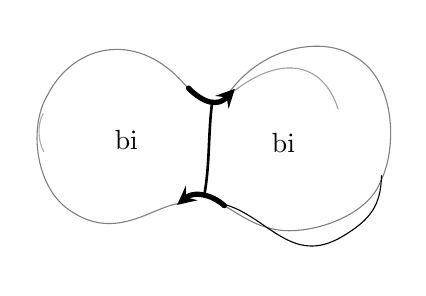
\begin{tikzpicture}[x=.0095cm,y=-.0095cm,line cap=round,line join=round]
  \draw[gray] (278,145) .. controls (213,64) and (125,84) .. (90,153) .. controls (64,195) and (73,279) .. (122,309) .. controls (181,348) and (228,304) .. (265,298);
  \draw[gray!65] (84,178) .. controls (75,194) and (78,218) .. (85,229);
  \draw[gray] (333,149) .. controls (380,86) and (458,76) .. (497,100) .. controls (556,130) and (557,225) .. (535,268) .. controls (517,317) and (438,341) .. (395,333) .. controls (365,328) and (344,311) .. (319,297);
  \draw[gray!75] (339,148) .. controls (402,99) and (458,109) .. (478,172);
  \draw (325,299) .. controls (384,315) and (416,383) .. (484,342) .. controls (521,320) and (535,301) .. (536,261);
  \draw[line width=.95pt] (310,161) .. controls (304,204) and (307,246) .. (299,288);
  \draw[line width=1.9pt,->,>=stealth] (278,144) .. controls (298,164) and (317,169) .. (340,145);
  \draw[line width=1.9pt,->,>=stealth] (326,301) .. controls (308,285) and (285,282) .. (263,300);
  \node at (195,213) {bi}; \node at (405,217) {bi};
\end{tikzpicture}}
\unsure{attachement|Attachement} de deux arêtes \deleted{\unsure{birives|bifidées}}\unsure{bifides} : on trouve \deleted{deux} \inserted{paire d'}arêtes \deleted{opposées} \inserted{$\unsure{a|e},a'$ \uline{\unsure{birives|monorives|bivives}}} qui sont tels que $(a,\omega)\unsure{,}(a',\omega)$ et $(a,\bar{\omega}),(a',\bar{\omega})$ sont des \inserted{\deleted{\unsure{paire|paires}} d'}arcs associés, \deleted{\unsure{mais}} \[\begin{aligned}f&=f'\unsure{+|-}f''-2\\ g&=g'+g''\end{aligned}\ \left|\begin{aligned}&4\ \text{faces}\\ &\text{deviennent }2\end{aligned}\right.\]
\end{minipage}\hfill\begin{minipage}[t]{.50\linewidth}
\figure{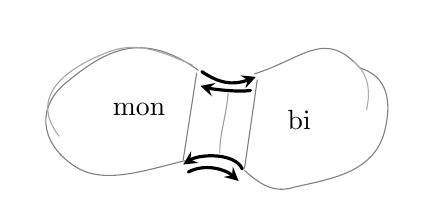
\begin{tikzpicture}[x=.0095cm,y=-.0095cm,line cap=round,line join=round]
  \draw[gray] (1075,177) .. controls (1000,123) and (951,151) .. (902,191) .. controls (857,225) and (864,274) .. (908,304) .. controls (946,331) and (1000,312) .. (1057,298);
  \draw[gray!70] (889,265) .. controls (848,212) and (898,174) .. (957,152) .. controls (995,138) and (1031,154) .. (1067,170);
  \draw[gray] (1150,182) .. controls (1215,162) and (1244,121) .. (1291,174) .. controls (1320,183) and (1337,207) .. (1324,259) .. controls (1309,317) and (1245,323) .. (1201,334) .. controls (1176,341) and (1158,330) .. (1137,311);
  \draw[gray!65] (1282,165) .. controls (1304,182) and (1305,207) .. (1300,230);
  \draw[gray] (1073,181) -- (1055,297) (1154,190) -- (1137,308); \draw[gray!75] (1115,208) .. controls (1113,237) and (1103,264) .. (1104,288);
  \draw[line width=1.15pt,->,>=stealth] (1080,179) .. controls (1102,194) and (1121,198) .. (1152,186);
  \draw[line width=1.15pt,->,>=stealth] (1145,204) .. controls (1129,207) and (1092,202) .. (1078,198);
  \draw[line width=1.15pt,->,>=stealth] (1134,309) .. controls (1124,287) and (1077,289) .. (1055,303);
  \draw[line width=1.15pt,->,>=stealth] (1062,313) .. controls (1085,301) and (1112,310) .. (1129,325);
  \node at (996,230) {mon}; \node at (1210,244) {bi};
\end{tikzpicture}}
Attachement de deux arêtes, l'une \unsure{monorive|monovive}, l'autre birive. On trouve \unsure{paire|pair} d'arêtes $\{a,a'\}$ \unsure{(}\deleted{\unsure{birives}}\inserted{monorives}) incidentes \unsure{:|à} une \unsure{$=$} face \[\begin{aligned}f^{\unsure{\ast|\prime}}&=f'+f''-2\\ g&=g'\unsure{-|+}g''\end{aligned}\ \left|\begin{aligned}&\text{\unsure{trois|deux} faces}\\ &\text{deviennent }1\end{aligned}\right.\]
\end{minipage}

\figure{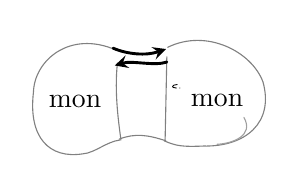
\begin{tikzpicture}[x=.011cm,y=-.011cm,line cap=round,line join=round]
  \draw[gray] (775,937) .. controls (722,914) and (681,949) .. (680,986) .. controls (674,1038) and (698,1063) .. (737,1057) .. controls (751,1056) and (764,1043) .. (780,1041);
  \draw[gray] (835,934) .. controls (880,912) and (932,939) .. (945,974) .. controls (958,1021) and (925,1049) .. (876,1048) .. controls (852,1049) and (845,1048) .. (831,1042);
  \draw[gray!75] (923,1015) .. controls (935,1036) and (910,1045) .. (892,1046);
  \draw[gray] (777,952) .. controls (773,987) and (779,1025) .. (781,1041) (834,945) -- (832,1042) (779,1040) .. controls (797,1033) and (812,1035) .. (833,1042);
  \draw[line width=1.05pt,->,>=stealth] (772,935) .. controls (788,942) and (810,944) .. (833,936);
  \draw[line width=1.05pt,->,>=stealth] (834,951) .. controls (820,956) and (794,949) .. (774,955);
  \node at (728,997) {mon}; \node at (892,995) {mon}; \draw[line width=.32pt] (846,977) .. controls (840,977) and (838,981) .. (845,981); \fill (849,981) circle (.6);
\end{tikzpicture}}
Attachement de deux arêtes \deleted{\unsure{bifides|bifidées}}\unsure{monorives} on trouve \deleted{deux} paire d'arêtes monorives, incidentes à des faces distinctes

\noindent\begin{minipage}[c]{.46\linewidth}
\[\begin{aligned}f&=f'+f''\\ \underline{g}&=g'+g''-1\end{aligned}\]
\end{minipage}\hfill\begin{minipage}[c]{.51\linewidth}
\figure{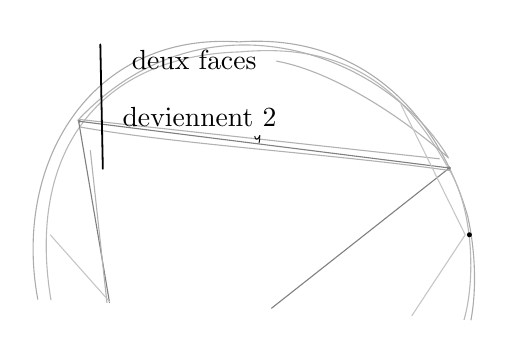
\begin{tikzpicture}[x=.0106cm,y=-.0106cm,line cap=round,line join=round]
  \clip (946,1308) -- (1489,1308) -- (1489,1659) -- (945,1633) -- cycle;
  \draw[gray!65] (958,1638) .. controls (925,1473) and (1019,1313) .. (1198,1325) .. controls (1335,1315) and (1433,1400) .. (1472,1534) .. controls (1483,1584) and (1482,1633) .. (1474,1667);
  \draw[gray!55] (975,1646) .. controls (940,1465) and (1024,1342) .. (1199,1337) .. controls (1321,1326) and (1392,1374) .. (1448,1475) .. controls (1478,1521) and (1483,1611) .. (1466,1663);
  \draw[gray!60] (1005,1419) .. controls (1156,1258) and (1373,1337) .. (1449,1464) .. controls (1396,1417) and (1313,1361) .. (1243,1348);
  \draw[gray] (1006,1420) -- (1450,1476) -- (1237,1644) (1006,1420) -- (1043,1637);
  \draw[gray!60] (1008,1427) .. controls (1126,1448) and (1310,1459) .. (1450,1479) (1008,1418) -- (1438,1465) (1020,1455) -- (1040,1638);
  \draw[gray!45] (972,1556) -- (1043,1636) (1392,1400) -- (1469,1556) -- (1405,1653);
  \fill[gray] (1007,1420) circle (2) (1450,1476) circle (2); \fill (1474,1556) circle (3);
  \draw[line width=.65pt] (1032,1328) -- (1035,1477);
  \node[anchor=west] at (1058,1346) {deux faces};
  \node[anchor=west] at (1047,1415) {deviennent $2$};
  \draw[line width=.33pt] (1217,1438) .. controls (1217,1441) and (1220,1445) .. (1223,1437) .. controls (1224,1440) and (1222,1444) .. (1222,1446);
\end{tikzpicture}}
\end{minipage}
% archive sheet number: 53

\scanpage{55}
\figure{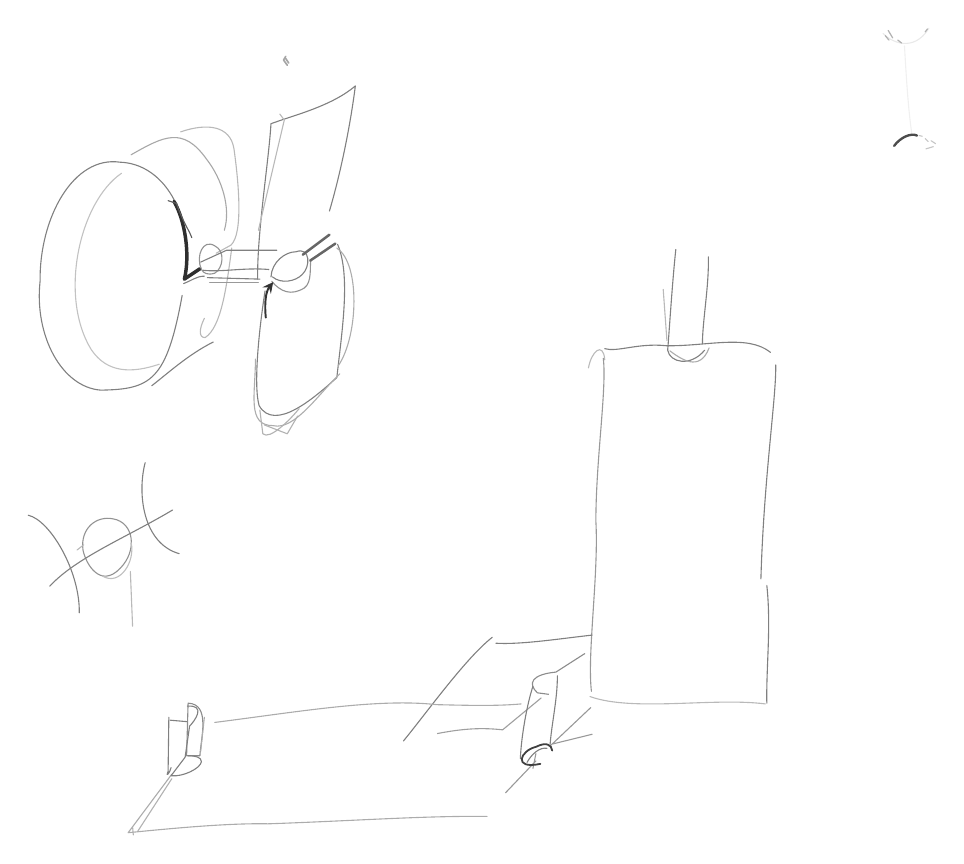
\begin{tikzpicture}[x=.0094cm,y=-.0094cm,line cap=round,line join=round]
  % Ink visible through the sheet from the opposite-face drawings on scan 54.
  \draw[gray!17] (1341,151) .. controls (1351,162) and (1382,178) .. (1403,144);
  \draw[gray!60,line width=.45pt] (1344,154) -- (1349,160) (1348,147) -- (1354,157) (1361,160) -- (1366,164) (1398,149) -- (1401,145);
  \draw[gray!12] (1370,168) .. controls (1372,203) and (1375,255) .. (1380,287);
  \draw[black!70,line width=.85pt] (1356,303) .. controls (1364,292) and (1378,285) .. (1387,289);
  \draw[gray!45] (1390,289) -- (1394,290) (1398,293) -- (1402,297) (1406,296) -- (1412,300) (1399,307) -- (1409,304);
  \draw[gray!70,line width=.6pt] (534,182) -- (531,187) -- (536,194) (534,185) -- (538,191);
  % Upper left
  \draw[gray] (398,480) .. controls (410,393) and (368,327) .. (310,325) .. controls (247,316) and (201,400) .. (202,486) .. controls (194,559) and (231,629) .. (284,633) .. controls (352,632) and (373,620) .. (394,505);
  \draw[gray!48] (312,340) .. controls (255,379) and (227,506) .. (271,578) .. controls (293,611) and (327,610) .. (363,598);
  \draw[gray!68] (325,315) .. controls (369,290) and (395,276) .. (427,321) .. controls (448,348) and (460,387) .. (451,417);
  \draw[gray!55] (392,284) .. controls (427,272) and (459,275) .. (464,307) .. controls (470,350) and (477,421) .. (460,437) -- (440,448);
  \draw[gray!55] (461,441) .. controls (454,493) and (447,548) .. (425,562) .. controls (416,562) and (417,550) .. (424,536);
  \draw[gray] (436,568) .. controls (402,585) and (375,610) .. (353,627);
  \draw[black!82,line width=1.25pt] (383,378) .. controls (398,404) and (405,450) .. (397,483) -- (418,469);
  \draw[black!64] (375,377) -- (387,381) (386,380) .. controls (395,406) and (404,418) .. (407,427);
  \draw[gray] (396,489) .. controls (405,486) and (413,479) .. (424,479);
  \draw[gray!85] (420,470) .. controls (412,452) and (422,428) .. (438,438) .. controls (453,445) and (449,469) .. (438,475) .. controls (428,478) and (423,475) .. (420,470);
  \draw[gray] (419,460) -- (454,444) -- (522,444) (422,471) .. controls (447,474) and (478,467) .. (511,470) (428,481) -- (499,483);
  \draw[gray!80] (431,487) -- (497,487);
  \draw[gray] (514,480) .. controls (515,460) and (533,446) .. (548,446) .. controls (567,439) and (568,466) .. (556,477) .. controls (547,486) and (528,490) .. (516,480);
  \draw[gray!85] (515,486) .. controls (527,500) and (541,506) .. (559,495) .. controls (570,487) and (566,466) .. (568,457);
  \draw[black!60,line width=.9pt] (557,450) -- (593,423) (567,458) -- (601,435);
  \draw[gray] (496,483) .. controls (495,421) and (511,324) .. (514,273) .. controls (547,261) and (596,249) .. (628,222) .. controls (621,277) and (608,340) .. (593,391);
  \draw[gray!55] (497,417) -- (532,268) -- (526,260);
  \draw[gray] (506,499) .. controls (498,550) and (490,626) .. (498,654) .. controls (519,690) and (572,644) .. (603,616) .. controls (610,552) and (622,478) .. (604,436);
  \draw[gray!64] (603,441) .. controls (635,462) and (632,560) .. (605,600) (493,591) .. controls (493,639) and (481,681) .. (517,681) .. controls (546,688) and (579,637) .. (607,611);
  \draw[gray!60] (499,660) -- (503,692) .. controls (512,701) and (540,673) .. (552,658) (505,680) -- (536,692) -- (550,668);
  \draw[black!80,line width=.7pt,->,>=stealth] (507,535) .. controls (505,516) and (507,500) .. (517,487);
  % Smaller sketch beneath the oval
  \draw[gray] (186,802) .. controls (216,809) and (256,878) .. (255,934);
  \draw[gray] (344,731) .. controls (333,773) and (341,840) .. (390,854);
  \draw[gray!85] (260,849) .. controls (256,820) and (278,802) .. (301,807) .. controls (329,812) and (334,850) .. (310,874) .. controls (284,901) and (264,869) .. (260,849);
  \draw[gray!50] (286,884) .. controls (310,899) and (331,864) .. (325,839);
  \draw[gray] (215,898) .. controls (251,859) and (319,832) .. (381,795);
  \draw[gray!55] (252,849) -- (261,842) (324,878) -- (327,952);
  % The upright sheet, its top return and the sloping lower sheet
  \draw[gray] (965,577) .. controls (982,582) and (1010,569) .. (1048,573) .. controls (1103,574) and (1158,557) .. (1189,582);
  \draw[gray] (1196,599) .. controls (1197,642) and (1180,750) .. (1176,888) (1184,897) .. controls (1190,953) and (1183,1007) .. (1184,1056);
  \draw[gray!80] (963,590) .. controls (968,630) and (953,727) .. (953,810) .. controls (957,881) and (941,990) .. (947,1040);
  \draw[gray!55] (945,1047) .. controls (1003,1068) and (1112,1048) .. (1182,1057);
  \draw[gray!55] (943,603) .. controls (947,580) and (963,567) .. (965,592) (1044,497) -- (1049,566);
  \draw[gray] (1061,443) .. controls (1056,490) and (1052,556) .. (1050,579) .. controls (1053,596) and (1081,602) .. (1100,579);
  \draw[gray] (1105,453) .. controls (1106,492) and (1097,540) .. (1097,570);
  \draw[gray!65] (1053,580) .. controls (1067,590) and (1093,610) .. (1106,576);
  \draw[gray] (693,1107) .. controls (722,1072) and (777,995) .. (813,967) (818,975) .. controls (852,977) and (903,969) .. (948,964);
  \draw[gray!75] (739,1097) .. controls (775,1090) and (800,1089) .. (827,1092) -- (879,1049);
  \draw[gray!65] (438,1082) .. controls (549,1068) and (657,1049) .. (738,1058) .. controls (782,1059) and (819,1060) .. (852,1057);
  \draw[gray!65] (380,1152) -- (321,1231) .. controls (391,1224) and (460,1218) .. (510,1219) .. controls (626,1215) and (722,1208) .. (806,1209);
  \draw[gray!60] (327,1223) -- (328,1234) (334,1229) -- (380,1158);
  \draw[gray] (376,1075) -- (375,1148) .. controls (371,1158) and (378,1149) .. (379,1143) (378,1079) -- (401,1081);
  \draw[gray!90] (402,1056) .. controls (433,1057) and (419,1104) .. (418,1127) -- (400,1127) -- (402,1056);
  \draw[gray] (401,1060) .. controls (427,1058) and (411,1080) .. (404,1087) -- (398,1129) -- (379,1154) .. controls (395,1156) and (419,1144) .. (420,1135) .. controls (420,1129) and (412,1127) .. (402,1127);
  \draw[gray!65] (424,1075) -- (419,1121);
  \draw[gray!90] (938,989) -- (899,1014) .. controls (867,1017) and (860,1029) .. (874,1042) -- (889,1044);
  \draw[gray] (901,1019) .. controls (901,1052) and (893,1084) .. (891,1114) (868,1033) .. controls (860,1057) and (852,1102) .. (851,1131);
  \draw[gray!80] (831,1177) -- (872,1134) (868,1144) -- (872,1124) (891,1114) -- (946,1062) (895,1111) -- (948,1098);
  \draw[black!75,line width=.65pt] (878,1138) .. controls (840,1146) and (851,1120) .. (872,1115) .. controls (886,1108) and (893,1112) .. (894,1120);
  \draw[gray] (860,1136) .. controls (866,1125) and (877,1115) .. (887,1117);
\end{tikzpicture}}
% archive sheet number: 54

